

\newpage
\tikz[remember picture,overlay]\node[opacity=1,inner sep=0pt] at (current page.center)%
{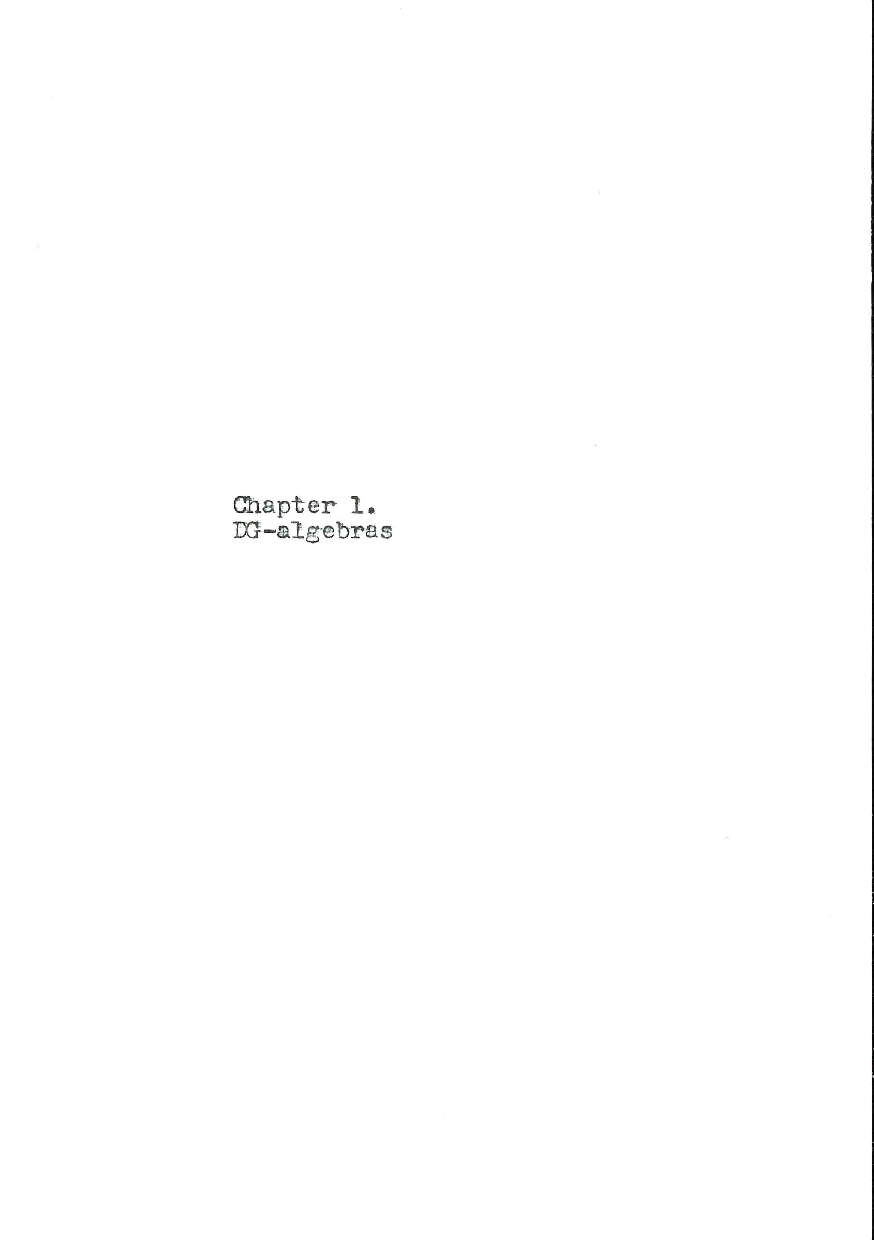
\includegraphics[%
clip,
width=1.05\paperwidth,
height=1.05\paperheight
]{chaptertitles/ch1.pdf}};

\clearpage

\subsection*{Description}

The main result of the first paper concerns the behaviour of a class of objects when a parameter is increased. At low values the objects act very topological --- which in spirit acts like fluidity, movement, deformation. Increasing the parameter makes the objects behave more and more algebraic, which is more rigid, less fluid, more staccato, more mechanical. Above a certain threshold, the behaviour of the objects is completely algebraic, which is depicted using only straight lines, while the topological behaviour at lower values is depicted with more flowing curved lines. 

The colors have no mathematical meaning, and are there only to add visual interst, and to connect to the colors of the papers. 


\newpage